%Descripción de la empresa
\chapter{Descripción del Instituto Receptor}\label{sec:capitulo2}
\thispagestyle{empty}

\begingroup
\rightskip0.5cm
\small
\endgroup
\begin{wrapfigure}{r}{10cm}
	\begin{center}
		
\includegraphics[scale=.6]{Imagenes/tecnaliar}
		\caption{Logo del TECNALIA \textit{ Research \& Innovation}}
		\label{fig:tecnaliar}
	\end{center}
\end{wrapfigure}
El instituo receptor del presente trabajo, TECNALIA \textit{Research \& Innovation} (Figura \ref{fig:tecnaliar}) es el primer centro privado de investigación de España, y uno de los más relevantes de Europa en general. Con sus 22 sedes distribuidas por todo el mundo buscan identificar y desarrollar distintas soluciones tecnológicas integrales, con creatividad e imaginación para más de 4.000 clientes, haciendo honor a su lema Inspiring Business, lema que tiene el significado de saber imaginar. Este concepto es producto de la síntesis de imaginar y hacer realidad, donde imaginar para TECNALIA supone tener ideas para ayudar a la sociedad y hacer realidad, aportar soluciones a los problemas \footnote{ http://www.tecnalia.es/proyectos-item/tecnalia-research-innovation }.\\    

\par A pesar de ser un centro de investigación relativamente nuevo, el mismo recoge la experiencia, el recorrido y las fortalezas de varias organizaciones con un extenso curriculum\footnote{https://www.tecnalia.com/es/tecnalia/historia.htm}, es por eso que a continuación se procederá a relatar de forma breve la historia de este centro, así como de la corporación TECNALIA, de la cual es integrante.

\section{Reseña Histórica}
TECNALIA Resarch \& Innovation nace en el 2010 como la unión de 8 empresas (Figura \ref{fig:tecnaliah}), unidas, con la intensión de colaborar y desarrollar nuevas oportunidades de progreso.\\  
\begin{figure}[!h]
	\centering
		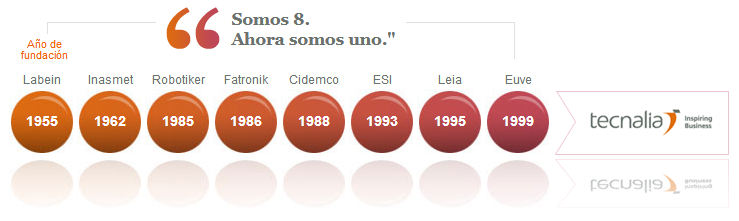
\includegraphics[scale=0.7]{Imagenes/tecnaliah}
		\caption[Empresas que conforman TECNALIA \textit{Research \& Innovation}, for L0F]{Empresas que conforman TECNALIA \textit{Research \& Innovation} \protect\footnotemark}
		\label{fig:tecnaliah}
	\end{figure}	  
\footnotetext{ https://www.tecnalia.com/es/tecnalia/historia.htm}
\par A su vez, TECNALIA junto con los centros tecnológicos, Azti y Neiker conforman a la Corporación Tecnalia, cuyo objetivo es contrubuir al desarrollo del entorno económico y social a través del uso y fomento de la innovación tecnológica, mediante el estímulo y difusión de la investigación, en un contexto internacional \footnote{http://www.tecnalia.es/}. La corporación Tecnalia nació en el año 2001, a través de la iniciativa de Inasmet, Labein y Robotiker, los cuales apostaron por unir esfuerzos e impulsar a Tecnalia de tal forma que puediera alcanzar niveles superiores de competitividad en el mercado. A raíz de esta unión otros centros tecnológicos se fueron incorporando con el pasar de los años (Figura \ref{fig:ctecnalia}), dando forma a lo que se conoce hoy como Corporación Tecnalia.\\ 
\begin{figure}[!h]
	\centering
		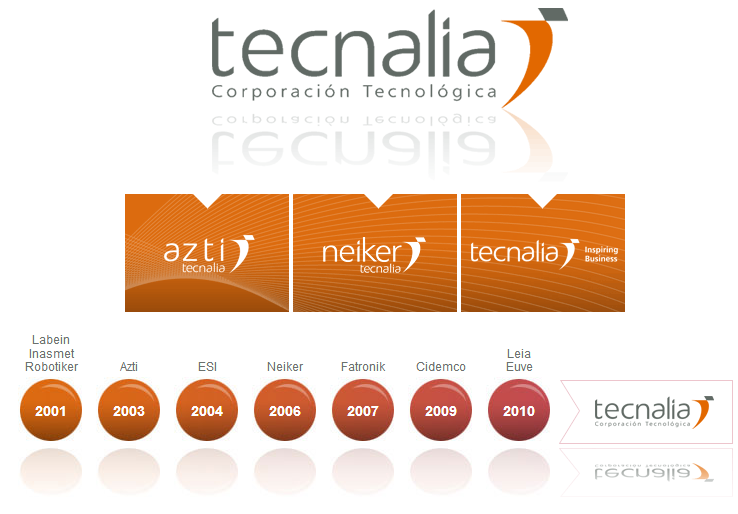
\includegraphics[scale=0.5]{Imagenes/ctecnalia}
		\caption[Empresas que conforman la Corporación Tecnalia,for L0F]{Empresas que conforman la Corporación Tecnalia \protect\footnotemark }
		\label{fig:ctecnalia}
	\end{figure}	  
\footnotetext{https://www.tecnalia.com/es/tecnalia/corporacion\-tecnalia.htm}
\section{Divisiones de TECNALIA \textit{Research \& Innovation} y Equipo de Automated Driving}
Dentro de la estructura de TECNALIA \textit{Research \& Innovation} se pueden encontrar 6 divisiones importantes:
\begin{itemize}
	\item Desarrollo sostenible.
	\item Tecnología de información y comunicación.
	\item Industria y transporte.
	\item Innovación y sociedad.
	\item Salud.
\end{itemize}
\par De estas divisiones se puede destacar la división de Industria y Transporte, la cual a su vez comprende varios focos de investigación, tales como: 
\begin{itemize}
	\item Tecnologías de fabricación  y trnasformación de materiales.
	\item Modelos predictivos de procesos de siderurgia y fundición .
	\item Tecnologías de materiales para transporte y espacio.
	\item Predicción, cotrol y mejora de características de los material.
	\item Homologación de materiales.
	\item Sistemas inteligentes de fabricación.
	\item Conducción autónoma.
\end{itemize}
\par De estos focos se resalta el de conducción autónoma, donde se desarrolló el presente trabajo. El mismo es un grupo multidisciplinario (Figura \ref{fig:equipo}) cuyo objetivo es  realizar investigaciones aplicadas a la conducción autónoma de vehículos eléctricos, esto, con el fin de poder realizar maniobras de forma segura, cómoda y eficiente en entornos urbanos e interurbanos. 
\begin{figure}[!h]
	\centering
		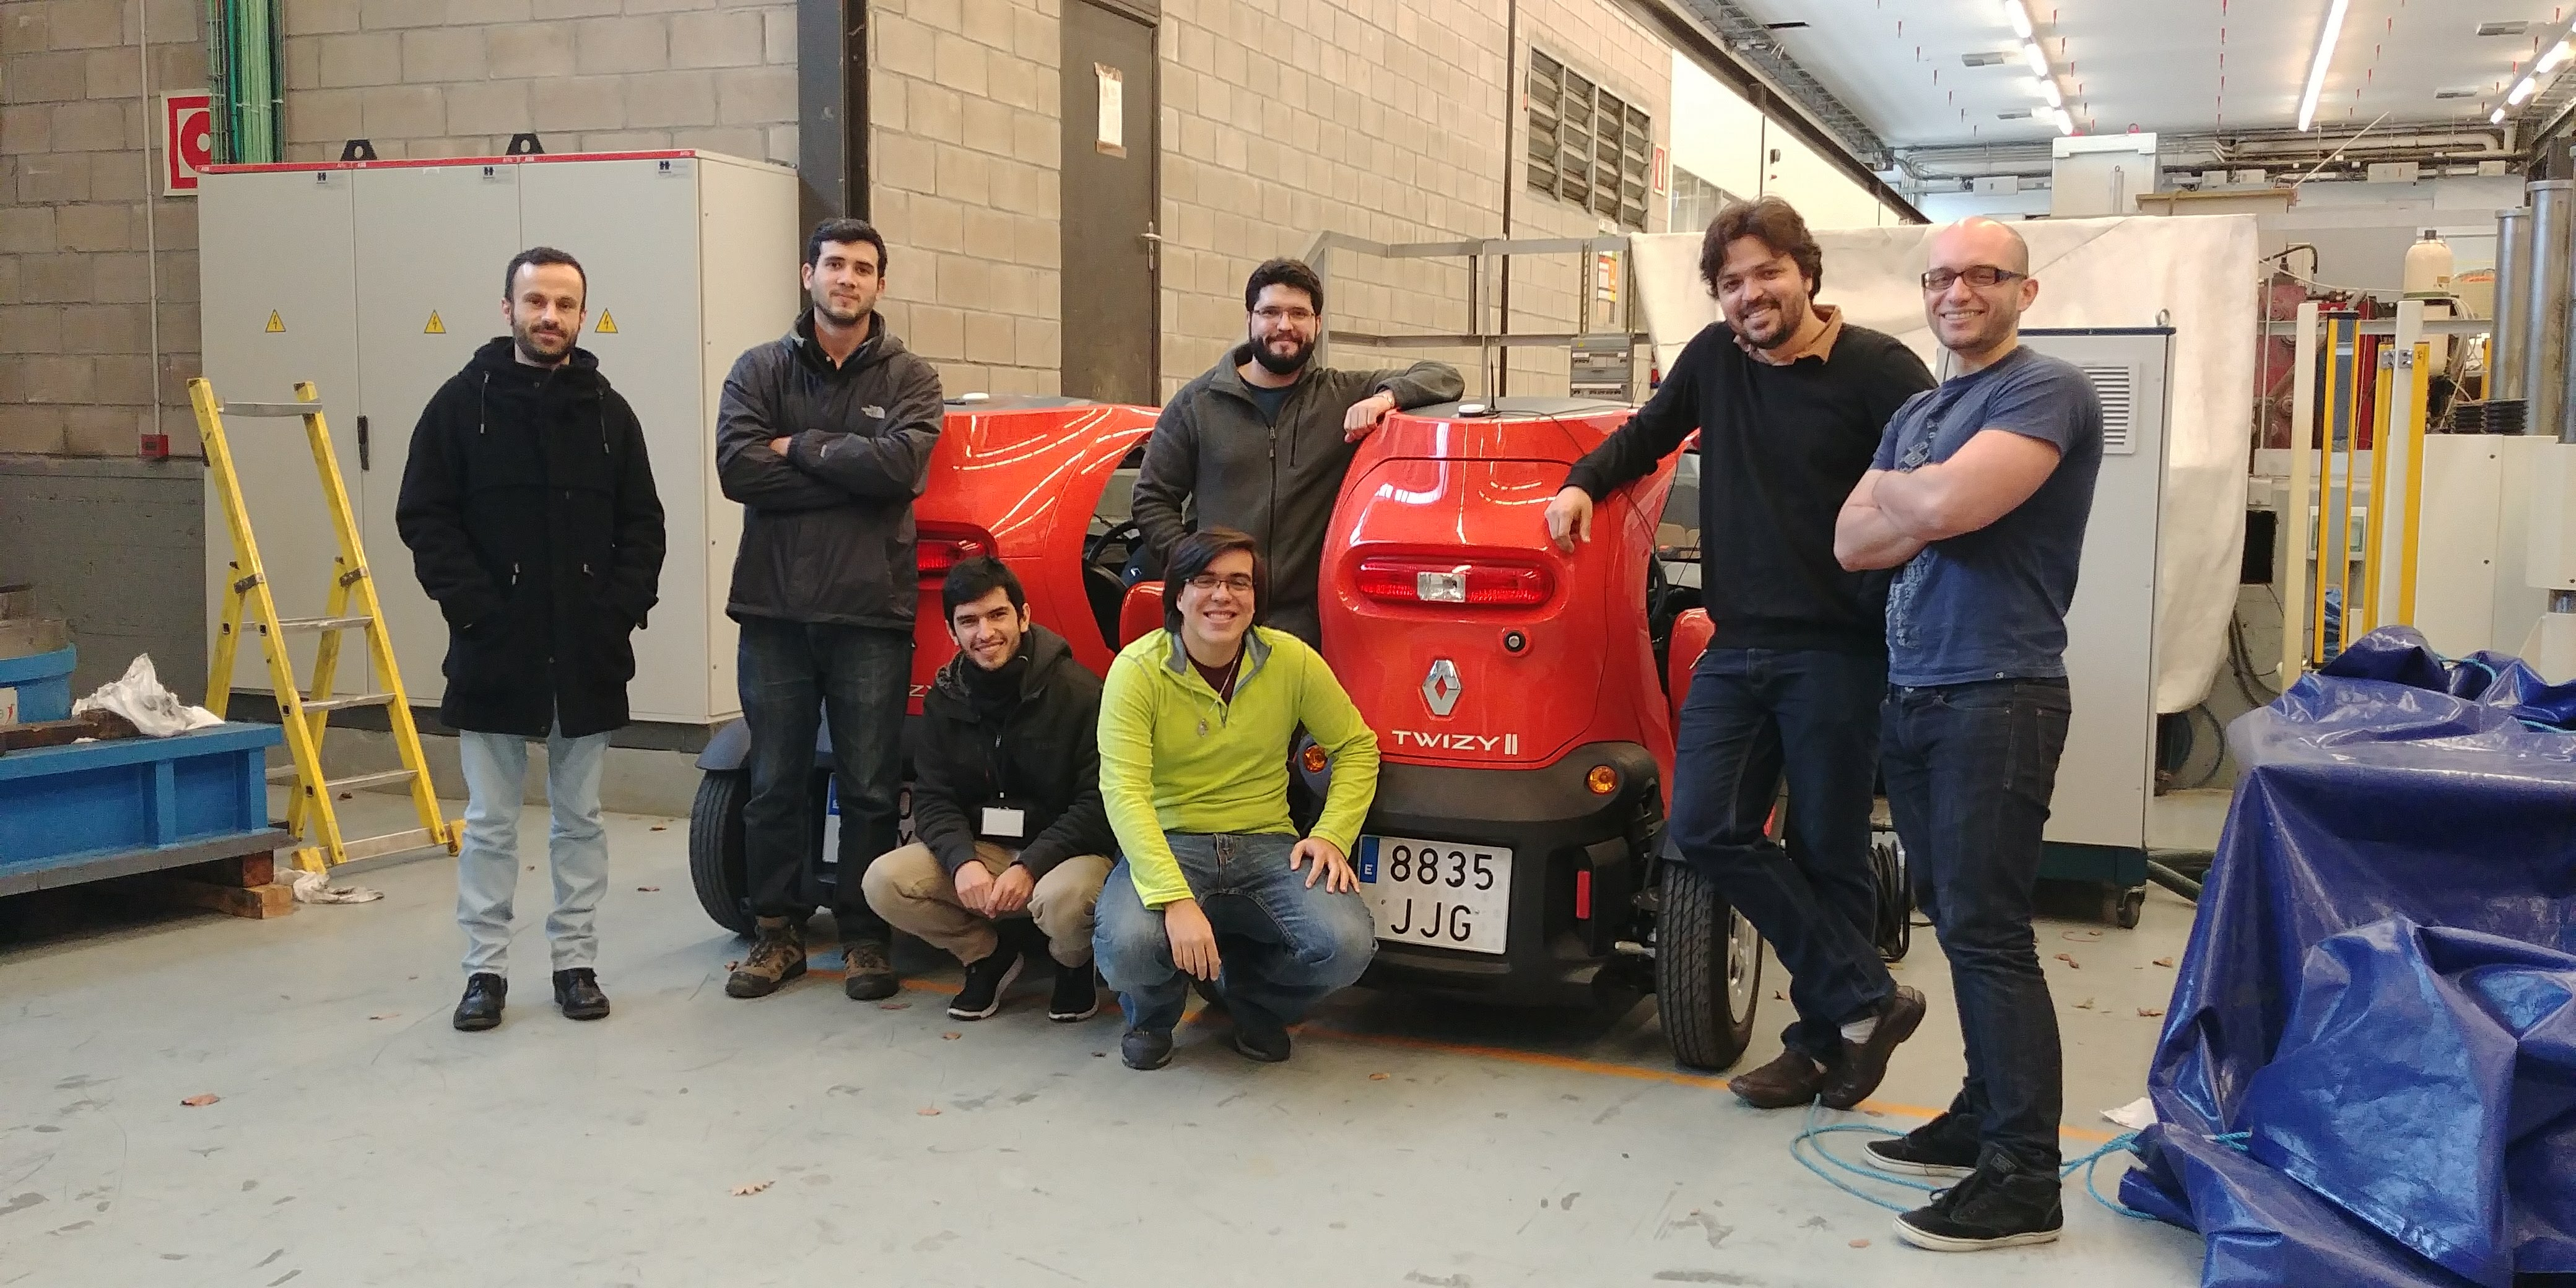
\includegraphics[scale=0.08]{Imagenes/equipo}
		\caption{Equipo de Automated Driving}
		\label{fig:equipo}
	\end{figure}	  
\subsection{Vehículos del Equipo}
Los vehículos utilizados por el equipo son dos Twizt Renault 80 (Figura \ref{fig:twizy}). Aparecieron por primera vez en el año 2009 en el salón del automóvil en Frankfurt, pero no fue si no hasta el 2011 que comenzó su producción \footnote{https://www.muyinteresante.es/innovacion/fotos/fotos-renault-twizy-coche-electrico-revolucionara-ciudades/fotos-parecido-smart\_\_\_1531}. Los Twizy disponen de un motor de 8 kW y 57 Nm, con una aceleración de 0 a 45 Km/h en 6,1 segundos, los mismos son vehículos eléctricos, que requieren una carga de 3 horas y 30 minutos, enchufados a una toma de 220 V, con 10 A\footnote{ http://www.renaulttwizy.org/renault-twizy-caracteristicas.php}.\\
\begin{figure}[!h]
	\centering
		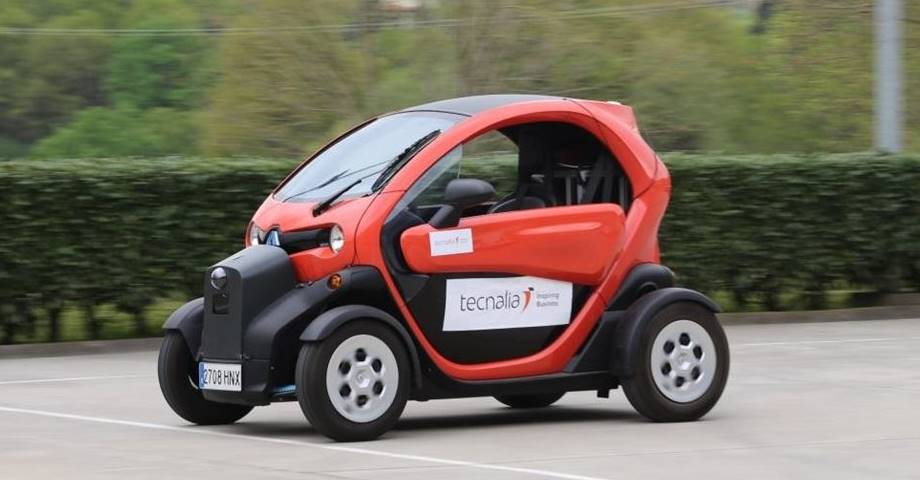
\includegraphics[scale=0.5]{Imagenes/twizy}
		\caption{Vehículo Twizy de TECNALIA}
		\label{fig:twizy}
	\end{figure}	  
\par Estos vehículos son instrumentados por la empresa española, Dirección de Tecnología Avanzada, DTA, la cual equipa los vehículos con actuadores y dispositivos electrónicos que permiten controlar los pedales y el volante del vehículo a través de Bus CAN. Esta comunicación es realizada a través de un PLC (del inglés, \textit{Programable Logic Contollers}) que sirve como interfaz entre la PC que implementa los algoritmos de conducción y los actuadores de vehículo. Cabe destacar que además de los componentes nombrados anteriormente los Twizy también fueron equipados con un GPS diferencial.\\  

\par A fines de este proyecto se resaltará el sistema de comunicación empleado en los Twizy, el cual consta de un router de la marca TP-Link conectado al CPU de cada vehículo (Figura \ref{fig:obus}), además de un dispositivo de red inalámbrico, empleado para conectar los vehículos a los routers.
\begin{figure}[!h]
	\centering
		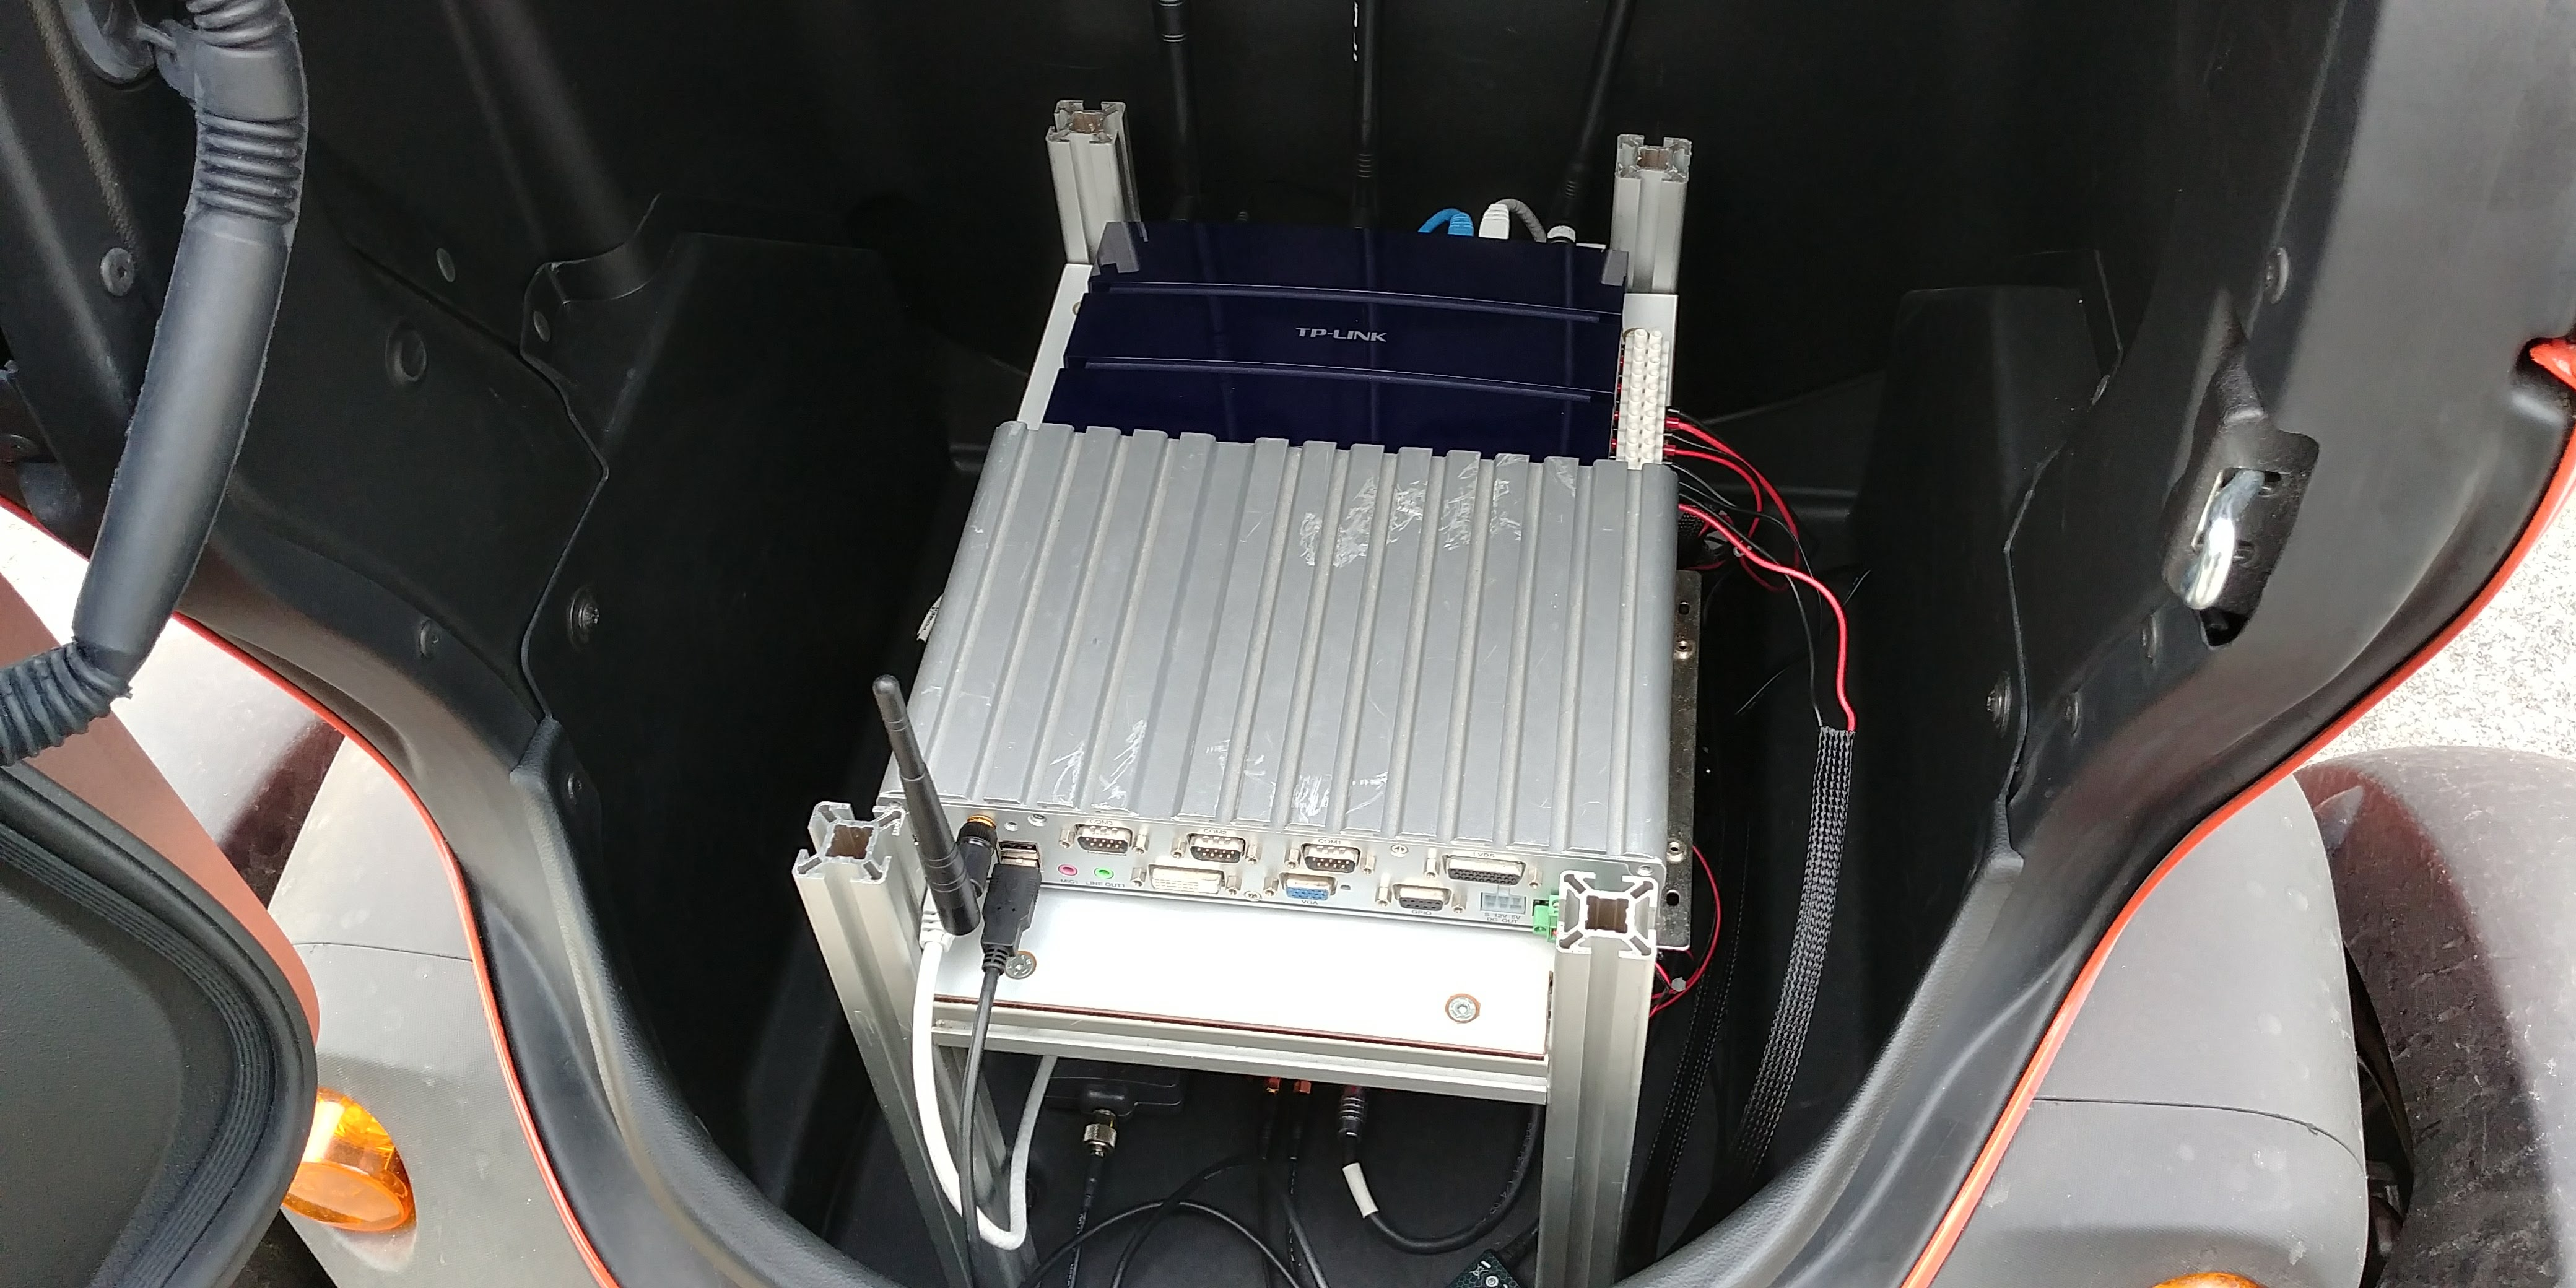
\includegraphics[scale=0.1]{Imagenes/obus}
		\caption{OBU del Twizy II}
		\label{fig:obus}
	\end{figure}	  
